\documentclass{standalone}
\usepackage{tikz}
\usetikzlibrary{patterns, positioning}
\usepackage[sfdefault]{ClearSans} %% option 'sfdefault' activates Clear Sans as the default text font
\usepackage[T1]{fontenc}

\begin{document}
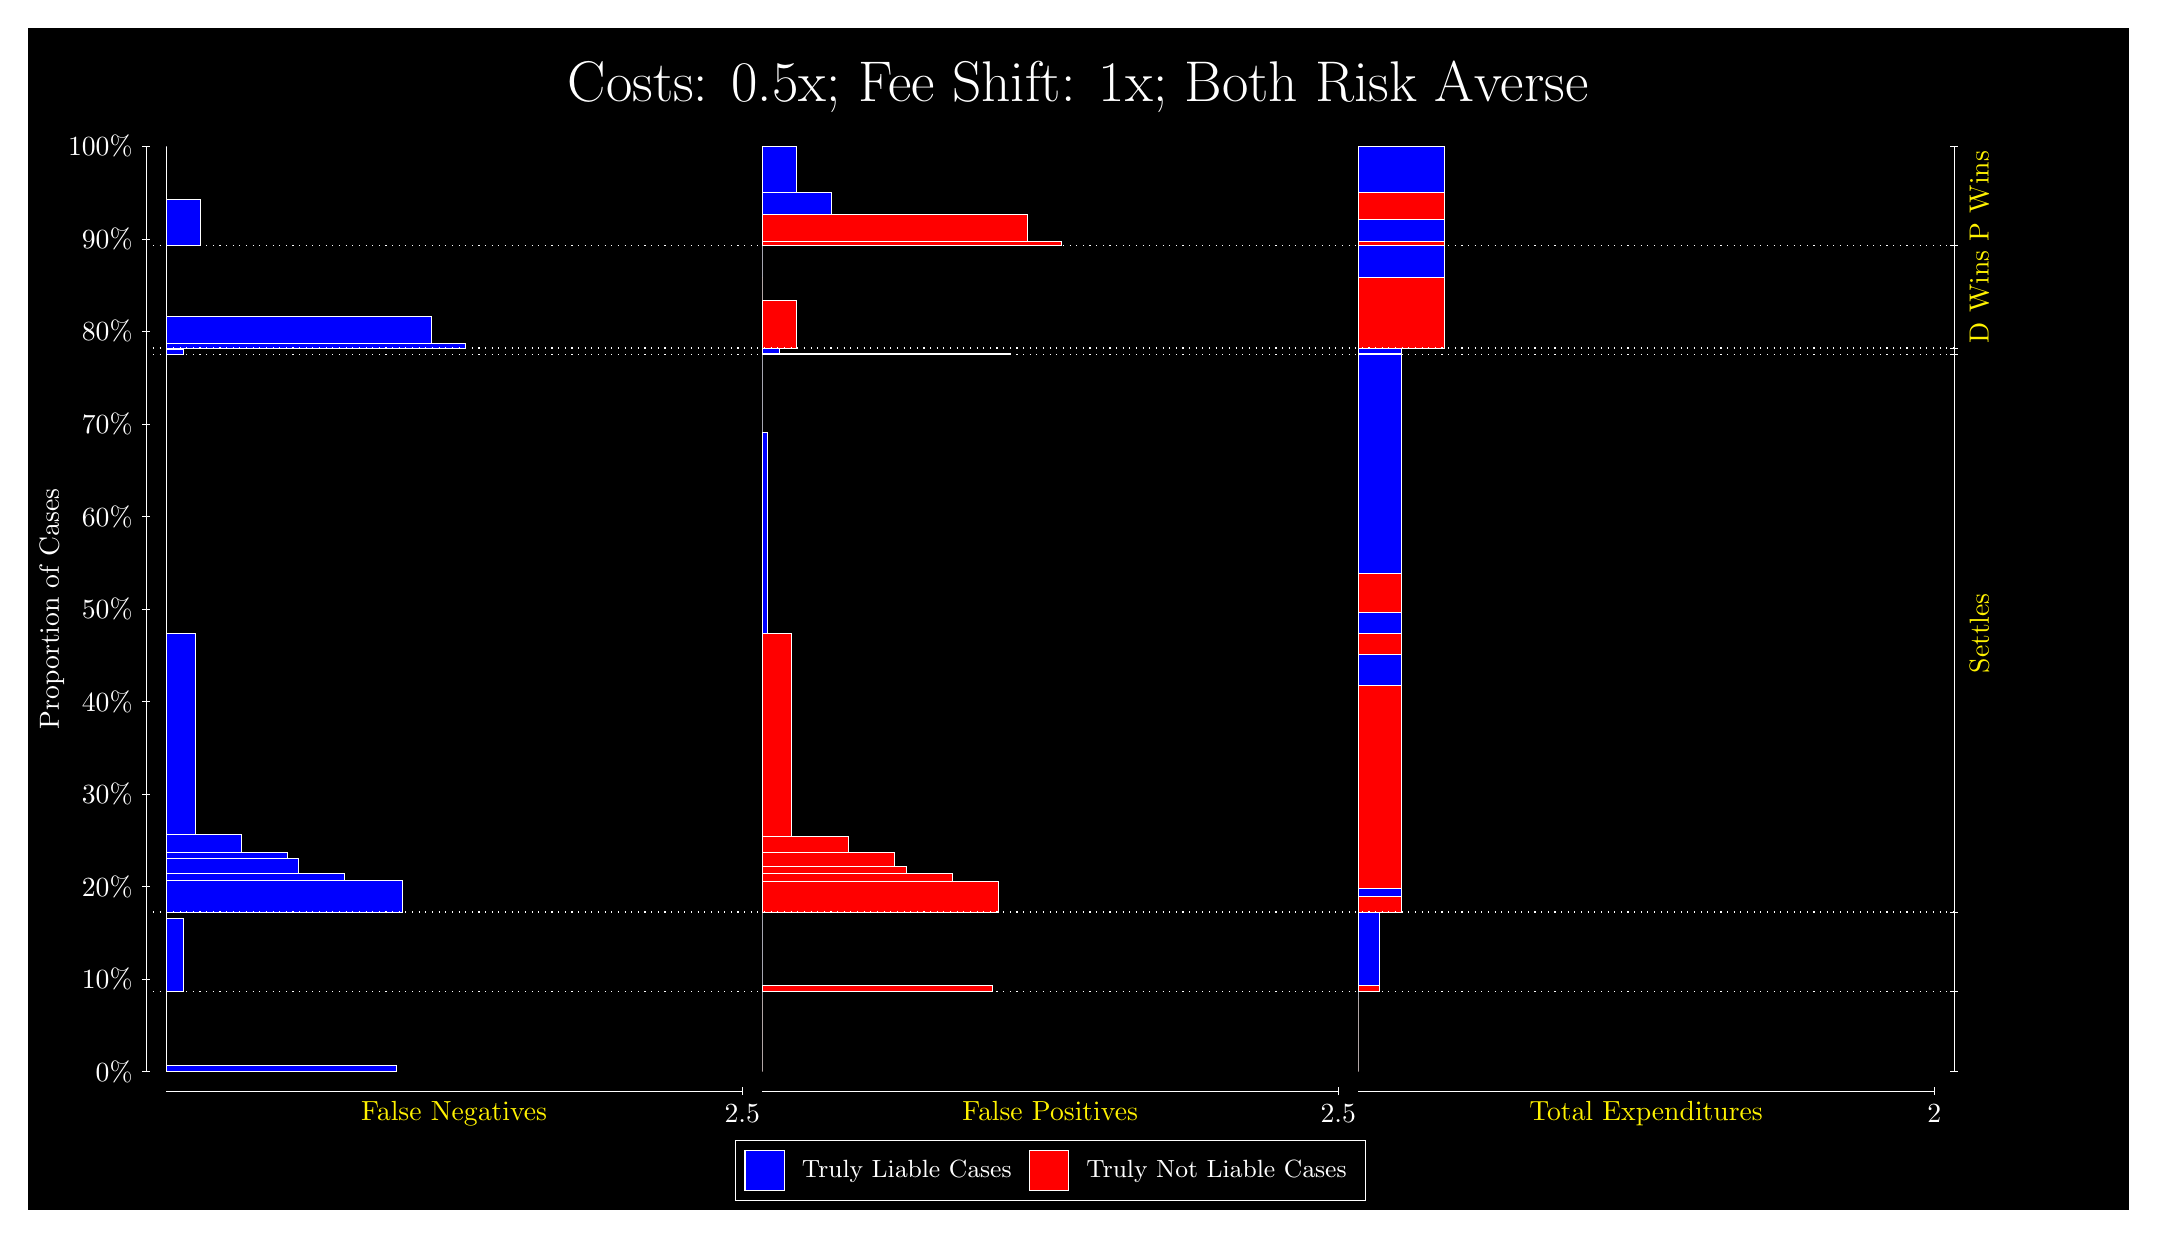
\begin{tikzpicture}
\draw[fill=black] (0,0) rectangle (26.667,15);
\draw[text=white] (0,13.5) rectangle (26.667,15) node[midway] {\huge Costs: 0.5x; Fee Shift: 1x; Both Risk Averse};
\draw[white, very thin] (1.5,1.75) -- (1.5,13.5);
\node[rotate=90, text=white, anchor=center] at (0.3, 7.625) {Proportion of Cases};
\draw[white, very thin] (1.45,1.75) -- (1.55,1.75);
\node[text=white, anchor=east] at (1.45, 1.75) {0\%};
\draw[white, very thin] (1.45,2.925) -- (1.55,2.925);
\node[text=white, anchor=east] at (1.45, 2.925) {10\%};
\draw[white, very thin] (1.45,4.1) -- (1.55,4.1);
\node[text=white, anchor=east] at (1.45, 4.1) {20\%};
\draw[white, very thin] (1.45,5.275) -- (1.55,5.275);
\node[text=white, anchor=east] at (1.45, 5.275) {30\%};
\draw[white, very thin] (1.45,6.45) -- (1.55,6.45);
\node[text=white, anchor=east] at (1.45, 6.45) {40\%};
\draw[white, very thin] (1.45,7.625) -- (1.55,7.625);
\node[text=white, anchor=east] at (1.45, 7.625) {50\%};
\draw[white, very thin] (1.45,8.8) -- (1.55,8.8);
\node[text=white, anchor=east] at (1.45, 8.8) {60\%};
\draw[white, very thin] (1.45,9.975) -- (1.55,9.975);
\node[text=white, anchor=east] at (1.45, 9.975) {70\%};
\draw[white, very thin] (1.45,11.15) -- (1.55,11.15);
\node[text=white, anchor=east] at (1.45, 11.15) {80\%};
\draw[white, very thin] (1.45,12.325) -- (1.55,12.325);
\node[text=white, anchor=east] at (1.45, 12.325) {90\%};
\draw[white, very thin] (1.45,13.5) -- (1.55,13.5);
\node[text=white, anchor=east] at (1.45, 13.5) {100\%};

\draw[white, very thin] (24.457,1.75) -- (24.457,13.5);
\draw[white, very thin] (24.407,1.75) -- (24.507,1.75);
\node[anchor=west] at (24.407, 1.75) {};
\draw[white, very thin] (24.407,2.7636) -- (24.507,2.7636);
\node[anchor=west] at (24.407, 2.7636) {};
\draw[white, very thin] (24.407,3.7759) -- (24.507,3.7759);
\node[anchor=west] at (24.407, 3.7759) {};
\draw[white, very thin] (24.407,10.855) -- (24.507,10.855);
\node[anchor=west] at (24.407, 10.855) {};
\draw[white, very thin] (24.407,10.939) -- (24.507,10.939);
\node[anchor=west] at (24.407, 10.939) {};
\draw[white, very thin] (24.407,12.24) -- (24.507,12.24);
\node[anchor=west] at (24.407, 12.24) {};
\draw[white, very thin] (24.407,13.5) -- (24.507,13.5);
\node[anchor=west] at (24.407, 13.5) {};

\draw[white, very thin, fill=blue] (1.75,1.75) rectangle (4.6775,1.832);
\draw[white, very thin, fill=red] (1.75,1.832) rectangle (1.75,2.7636);
\draw[white, very thin, fill=blue] (1.75,2.7636) rectangle (1.9696,3.6944);
\draw[white, very thin, fill=red] (1.75,3.6944) rectangle (1.75,3.7759);
\draw[white, very thin, fill=blue] (1.75,3.7759) rectangle (4.7507,4.1735);
\draw[white, very thin, fill=blue] (1.75,4.1735) rectangle (4.0188,4.2727);
\draw[white, very thin, fill=blue] (1.75,4.2727) rectangle (3.4333,4.4582);
\draw[white, very thin, fill=blue] (1.75,4.4582) rectangle (3.287,4.5392);
\draw[white, very thin, fill=blue] (1.75,4.5392) rectangle (2.7015,4.7577);
\draw[white, very thin, fill=blue] (1.75,4.7577) rectangle (2.1159,7.3162);
\draw[white, very thin, fill=red] (1.75,7.3162) rectangle (1.75,10.855);
\draw[white, very thin, fill=blue] (1.75,10.855) rectangle (1.9696,10.917);
\draw[white, very thin, fill=red] (1.75,10.917) rectangle (1.75,10.939);
\draw[white, very thin, fill=blue] (1.75,10.939) rectangle (5.5558,11.001);
\draw[white, very thin, fill=blue] (1.75,11.001) rectangle (5.1167,11.339);
\draw[white, very thin, fill=red] (1.75,11.339) rectangle (1.75,12.24);
\draw[white, very thin, fill=blue] (1.75,12.24) rectangle (2.1891,12.822);
\draw[white, very thin, fill=red] (1.75,12.822) rectangle (1.75,13.222);
\draw[white, very thin, fill=blue] (1.75,13.222) rectangle (1.75,13.5);
\draw[white, very thin, fill=red] (9.3189,1.75) rectangle (9.3189,2.6815);
\draw[white, very thin, fill=blue] (9.3189,2.6815) rectangle (9.3189,2.7636);
\draw[white, very thin, fill=red] (9.3189,2.7636) rectangle (12.246,2.845);
\draw[white, very thin, fill=blue] (9.3189,2.845) rectangle (9.3189,3.7759);
\draw[white, very thin, fill=red] (9.3189,3.7759) rectangle (12.32,4.1679);
\draw[white, very thin, fill=red] (9.3189,4.1679) rectangle (11.734,4.2726);
\draw[white, very thin, fill=red] (9.3189,4.2726) rectangle (11.149,4.352);
\draw[white, very thin, fill=red] (9.3189,4.352) rectangle (11.002,4.5375);
\draw[white, very thin, fill=red] (9.3189,4.5375) rectangle (10.417,4.7386);
\draw[white, very thin, fill=red] (9.3189,4.7386) rectangle (9.6848,7.3146);
\draw[white, very thin, fill=blue] (9.3189,7.3146) rectangle (9.3921,9.8731);
\draw[white, very thin, fill=blue] (9.3189,9.8731) rectangle (9.3189,10.855);
\draw[white, very thin, fill=red] (9.3189,10.855) rectangle (12.466,10.877);
\draw[white, very thin, fill=blue] (9.3189,10.877) rectangle (9.5384,10.939);
\draw[white, very thin, fill=red] (9.3189,10.939) rectangle (9.758,11.544);
\draw[white, very thin, fill=red] (9.3189,11.544) rectangle (9.3189,11.84);
\draw[white, very thin, fill=blue] (9.3189,11.84) rectangle (9.3189,12.24);
\draw[white, very thin, fill=red] (9.3189,12.24) rectangle (13.125,12.3);
\draw[white, very thin, fill=red] (9.3189,12.3) rectangle (12.686,12.64);
\draw[white, very thin, fill=blue] (9.3189,12.64) rectangle (10.197,12.918);
\draw[white, very thin, fill=blue] (9.3189,12.918) rectangle (9.758,13.5);
\draw[white, very thin, fill=red] (16.888,1.75) rectangle (16.888,2.6815);
\draw[white, very thin, fill=blue] (16.888,2.6815) rectangle (16.888,2.7636);
\draw[white, very thin, fill=red] (16.888,2.7636) rectangle (17.162,2.845);
\draw[white, very thin, fill=blue] (16.888,2.845) rectangle (17.162,3.7759);
\draw[white, very thin, fill=red] (16.888,3.7759) rectangle (17.437,3.9771);
\draw[white, very thin, fill=blue] (16.888,3.9771) rectangle (17.437,4.0762);
\draw[white, very thin, fill=red] (16.888,4.0762) rectangle (17.437,6.6522);
\draw[white, very thin, fill=blue] (16.888,6.6522) rectangle (17.437,7.0498);
\draw[white, very thin, fill=red] (16.888,7.0498) rectangle (17.437,7.3146);
\draw[white, very thin, fill=blue] (16.888,7.3146) rectangle (17.437,7.5812);
\draw[white, very thin, fill=red] (16.888,7.5812) rectangle (17.437,8.0779);
\draw[white, very thin, fill=blue] (16.888,8.0779) rectangle (17.437,10.855);
\draw[white, very thin, fill=red] (16.888,10.855) rectangle (17.437,10.877);
\draw[white, very thin, fill=blue] (16.888,10.877) rectangle (17.437,10.939);
\draw[white, very thin, fill=red] (16.888,10.939) rectangle (17.986,11.84);
\draw[white, very thin, fill=blue] (16.888,11.84) rectangle (17.986,12.24);
\draw[white, very thin, fill=red] (16.888,12.24) rectangle (17.986,12.3);
\draw[white, very thin, fill=blue] (16.888,12.3) rectangle (17.986,12.578);
\draw[white, very thin, fill=red] (16.888,12.578) rectangle (17.986,12.918);
\draw[white, very thin, fill=blue] (16.888,12.918) rectangle (17.986,13.5);
\draw[white, dotted] (1.5,2.7636) -- (24.457,2.7636);
\draw[white, dotted] (1.5,3.7759) -- (24.457,3.7759);
\draw[white, dotted] (1.5,10.855) -- (24.457,10.855);
\draw[white, dotted] (1.5,10.939) -- (24.457,10.939);
\draw[white, dotted] (1.5,12.24) -- (24.457,12.24);
\draw[white, very thin] (1.75,1.5) -- (9.0689,1.5);
\node[text=yellow, anchor=north] at (5.4094, 1.5) {False Negatives};
\draw[white, very thin] (9.0689,1.45) -- (9.0689,1.55);
\node[text=white, anchor=north] at (9.0689, 1.45) {2.5};

\draw[white, very thin] (9.3189,1.5) -- (16.638,1.5);
\node[text=yellow, anchor=north] at (12.978, 1.5) {False Positives};
\draw[white, very thin] (16.638,1.45) -- (16.638,1.55);
\node[text=white, anchor=north] at (16.638, 1.45) {2.5};

\draw[white, very thin] (16.888,1.5) -- (24.207,1.5);
\node[text=yellow, anchor=north] at (20.547, 1.5) {Total Expenditures};
\draw[white, very thin] (24.207,1.45) -- (24.207,1.55);
\node[text=white, anchor=north] at (24.207, 1.45) {2};



\node[text=yellow, centered, rotate=90] at (24.777, 7.3154) {Settles};

\node[text=yellow, centered, rotate=90] at (24.777, 11.59) {D Wins};
\node[text=yellow, centered, rotate=90] at (24.777, 12.87) {P Wins};

\draw (12.978300999999998,1.5) node[draw=none] (baseCoordinate) {};
\begin{scope}[align=center]
        \matrix[scale=0.5, draw=white, below=0.5cm of baseCoordinate, nodes={draw}, column sep=0.1cm]{
            \node[rectangle, draw, minimum width=0.5cm, minimum height=0.5cm, fill=blue] {}; &
            \node[draw=none, font=\small, text=white] (B) {Truly Liable Cases}; &
            \node[rectangle, draw, minimum width=0.5cm, minimum height=0.5cm, fill=red] {}; &
            \node[draw=none, font=\small, text=white] (B) {Truly Not Liable Cases}; \\
            };
\end{scope}

\end{tikzpicture}
\end{document}